\section{Documentation}


\begin{frame}[fragile]{What You Will Learn:}
  \begin{itemize}
    \item Documenting your code using \emph{Sphinx}
    \item \emph{reStructuredText} (\reST/\texttt{RST}) syntax
    \item Using \emph{Read the Docs}
  \end{itemize}
\end{frame}


\begin{frame}[fragile]{Why Should We Document Our Code?}
  Well-documented code improves\dots
  \begin{itemize}
    \item Maintainability: Future developers, debugging, \dots
    \item Accessibility: Make your package easier to understand for new users
    \item Collaboration: Docs as a shared knowledge source
  \end{itemize}
\end{frame}

\subsection{Sphinx}
\begin{frame}[fragile]{
  What is Sphinx?
  \hfill
  \doc{https://www.sphinx-doc.org}{Sphinx}}
  \begin{itemize}
    \setlength{\itemsep}{1em}
    \item Open-source, extensible documentation generator written in Python
    \item Multiple output formats: \texttt{HTML}, \LaTeX{} (for \texttt{PDF}), \texttt{ePub}, and more\dots
    \item Creates cross-references within your project and across different projects
    \item Allows documentation using a mark-up language (\reST)
    \item Supports various docstring formats (some through extensions)
  \end{itemize}

  \vspace{1cm}
  There are also alternatives to Sphinx, like \emph{MkDocs} and \emph{pdoc}, but Sphinx can be considered the industry standard for Python docs.
\end{frame}


\begin{frame}[fragile]{Installation}
  Sphinx can be installed via standard package managers:
  \begin{itemize}
    \setlength{\itemsep}{1em}
    \item Installing from PyPI using \texttt{pip}:
    \begin{minted}{shell-session}
      $ pip install -U sphinx
    \end{minted}
    \item Conda/Mamba:
    \begin{minted}{shell-session}
      $ mamba install sphinx
    \end{minted}
    \begin{minted}{shell-session}
      $ conda install -c conda-forge sphinx
    \end{minted}

    \item Debian/Ubuntu using \texttt{apt}:
    \begin{minted}{shell-session}
      # apt install python3-sphinx
    \end{minted}

  \item Fedora Linux, RHEL, CentOS using \texttt{yum} or \texttt{dnf}:
    \begin{minted}{shell-session}
      # yum install python-sphinx
      # dnf install python-sphinx
    \end{minted}

    \item Homebrew:
      \begin{minted}{shell-session}
        $ brew install sphinx-doc
      \end{minted}
  \end{itemize}
\end{frame}

\begin{frame}[fragile]{Getting Started}
  \begin{minted}[escapeinside=||]{shell-session}
    $ sphinx-quickstart docs
    |\textcolor{cmauve}{> Separate source and build directories (y/n) [n]:}| y
    |\textcolor{cmauve}{> Project name:}| ...
    |\textcolor{cmauve}{> Author name(s):}| ...
    |\textcolor{cmauve}{> Project release []:}| ...
    |\textcolor{cmauve}{> Project language [en]:}| ...
  \end{minted}

  \begin{center}
  \pause
  \begin{minipage}{.45\textwidth}
  \adjustbox{max height=5.5cm}{%
    \begin{forest}
      for tree={dir tree}
      [docs, opened
        [build, closed]
        [source, opened
          [\_static, closed]
          [\_templates, closed]
          [conf.py, pythonfile]
          [index.rst, textfile]
        ]
        [make.bat, batchfile]
        [Makefile, makefile]
      ]
    \end{forest}
  }
  \end{minipage}
  \hfill
  \pause
  \begin{minipage}{.45\textwidth}
    \adjustbox{max height=5.5cm}{%
      \begin{forest}
        for tree={dir tree}
        [docs, opened
          [\_build, closed]
          [\_static, closed]
          [\_templates, closed]
          [conf.py, pythonfile]
          [index.rst, textfile]
          [make.bat, batchfile]
          [Makefile, makefile]
        ]
      \end{forest}
    }
  \end{minipage}
  \end{center}
\end{frame}
{
\setbeamercolor{description item}{fg=vertexDarkGrey}
\begin{frame}[fragile]{Breakdown of the Generated Structure}
  \begin{description}[labelwidth=\widthof{\faFolderOpen \texttt{\_templates}}]
    \setlength{\itemindent}{-4em}
    \item [\textcolor{dircolor}{\faFolderOpen} \texttt{build}:] Output directory for the docs.
    \item [\textcolor{dircolor}{\faFolderOpen} \texttt{\_static}:] Directory for static elements such as images, icons, or logos.
    \item [\textcolor{dircolor}{\faFolderOpen} \texttt{\_templates}:] Used to store \href{https://jinja.palletsprojects.com/en/stable/}{\texttt{Jinja}}
      templates for HTML page generation. %Also used by some Sphinx extensions.
    \item [\textcolor{vertexDarkRed}{\faFile*} \texttt{index.rst}:] Root document; contains the root of the table of contents tree.
      % Effectively your landing page in the HTML version.
    \item [\textcolor{vertexDarkRed}{\faPython} \texttt{conf.py}:] Main configuration file written in Python.
  \end{description}
\end{frame}
}

\begin{frame}[fragile]{Let's Build Our Docs}
  We will use the \texttt{Makefile} generated by \mintinline{shell-session}+sphinx-quickstart+ to build any format:
  \begin{minted}{shell-session}
    $ make <format>
  \end{minted}
  So, for the HTML version:
  \begin{minted}{shell-session}
    $ make html
  \end{minted}
  This will generate the HTML files for our docs inside the \texttt{build} directory.
  We can view the docs locally by running a Python HTTP server (in this case from inside the \texttt{docs} directory):
  \begin{minted}{shell-session}
    $ python -m http.server -d build/html [port]
  \end{minted}

  \begin{block}{Note}
    \mintinline{shell-session}+[port]+ is optional, see \mintinline{shell-session}+python -m http.server --help+.
  \end{block}
\end{frame}


\begin{frame}[fragile]{Preview}
\end{frame}

\begin{frame}[fragile]{Setting Up \texttt{conf.py}}
  The \texttt{conf.py} file generated by Sphinx should look something like this:
  \begin{block}{Code | \texttt{docs/conf.py}}
  \begin{minted}{python}
    # -- Project information ------------------------
    project = 'pyopp'
    copyright = '2025, Author'
    author = 'Author'
    release = 'v0.1'

    # -- General configuration ----------------------
    extensions = []

    templates_path = ['_templates']
    exclude_patterns = []

    # -- Options for HTML output --------------------
    html_theme = 'alabaster'
    html_static_path = ['_static']
  \end{minted}
  \end{block}
\end{frame}

\begin{frame}[fragile]{Setting Up \texttt{conf.py} | Project Information}
  When using a \texttt{pyproject.toml} file for our project, we automatically get the metadata
  from that file using \texttt{tomli} or \texttt{tomllib} (Python $\geqslant$ \texttt{3.11}):
  \begin{block}{Code | \texttt{docs/conf.py}}
  \footnotesize
  \begin{minted}{python}
    #!/usr/bin/env python3
    import datetime
    import sys
    from pathlib import Path

    import pyvisgen

    if sys.version_info < (3, 11):
        import tomli as tomllib
    else:
        import tomllib

    pyproject_path = Path(__file__).parent.parent.parent / "pyproject.toml"
    pyproject = tomllib.loads(pyproject_path.read_text())

    project = pyproject["project"]["name"]
    author = pyproject["project"]["authors"][0]["name"]
    copyright = "{}.  Last updated {}".format(
        author, datetime.datetime.now().strftime("%d %b %Y %H:%M")
    )
    python_requires = pyproject["project"]["requires-python"]
  \end{minted}
  \end{block}
\end{frame}


\begin{frame}[fragile]{Setting Up \texttt{conf.py} | General Configuration}
  Sphinx extensions add functionality and customization. The following extensions
  are some of the extensions we always use in our docs:
  \begin{block}{Code | \texttt{docs/conf.py}}
    \footnotesize
    \begin{minted}{python}
      extensions = [
          "sphinx.ext.autodoc",                # Imports modules and pulls in documentation from docstrings
          "sphinx.ext.intersphinx",            # Cross-references to other projects
          "sphinx.ext.coverage",               # Collects doc coverage stats
          "sphinx.ext.viewcode",               # Links to highlighted source code (i.e. "[source]" button)
          "sphinx_automodapi.automodapi",                    # Automatically generates module documentation
          "sphinx_automodapi.smart_resolver",                # Helps resolving some imports
          "numpydoc",                                        # Support for the NumPy docstring format
          "IPython.sphinxext.ipython_console_highlighting",  # Syntax highlighting of ipython prompts
          "sphinx_copybutton",                               # Adds a copybutton to code blocks
      ]
    \end{minted}
  \end{block}
\end{frame}

\begin{frame}[fragile]{Setting Up \texttt{conf.py} | General Configuration}
  Now we can set up some more settings for the extensions:
  \begin{block}{Code | \texttt{docs/conf.py}}
    \begin{minted}{python}
    # gets rid of some errors during build
    numpydoc_show_class_members = False
    numpydoc_class_members_toctree = False

    intersphinx_mapping = {
       "numpy": ("https://numpy.org/doc/stable", None),
       ...
    }

    suppress_warnings = ["intersphinx.external"]  # sometimes necessary

    templates_path = ["_templates"]
    exclude_patterns = ["build", "Thumbs.db", ".DS_Store", "changes", "*.log"]

    source_suffix = ".rst"  # Set .rst files as source files for docs
    master_doc = "index"    # index.rst as root file
  \end{minted}
  \end{block}
\end{frame}


\begin{frame}[fragile]{Setting Up \texttt{conf.py} | General Configuration}
    Some extensions are external and need to be installed separately in your environment:
    \begin{minted}{shell-session}
      $ mamba install sphinx-automodapi numpydoc pydata-sphinx-theme sphinx-copybutton
    \end{minted}
    or with \texttt{pip}
    \begin{minted}{shell-session}
      $ pip install sphinx-automodapi numpydoc pydata-sphinx-theme sphinx-copybutton
    \end{minted}
\end{frame}


\begin{frame}[fragile]{Setting Up \texttt{conf.py} | HTML And Theme Options}
  HTML options set the look of your docs. The Sphinx community has created a variety of
  themes you can choose from.
  \begin{block}{Code | \texttt{docs/conf.py}}
  \footnotesize
  \begin{minted}{python}
    html_theme = "pydata_sphinx_theme"            # Modern, widely used theme
    html_static_path = ["_static"]

    html_file_suffix = ".html"

    html_css_files = ["custom.css"]               # Custom CSS settings like colors or fonts

    html_favicon = "_static/favicon/favicon.ico"  # Icon file for browser tabs

    html_theme_options = {...}                    # Depends on the theme

    html_title = f"{project}"                     # e.g. your project name
    htmlhelp_basename = project + "docs"
  \end{minted}
  \end{block}
\end{frame}




\begin{frame}[fragile]{Filling the Docs With Some API References}
  We will create the API references (semi-)automatically in a few steps:
  \begin{columns}[onlytextwidth]
    \begin{column}{0.48\textwidth}
      \begin{enumerate}
        \item <1-> Copy the structure of your actual package
        \item <2-> Populate every subdirectory with a \texttt{index.rst}
        \item <3-> Create separate \texttt{.rst} files for every submodule
      \end{enumerate}
      \vspace{0.25cm}
      \begin{center}
        \adjustbox{max height=5cm}{%
          \begin{forest}
            for tree={dir tree}
            [package, opened
              [module1, opened
                [\_\_init\_\_.py, pythonfile]
                [submodule\_a.py, pythonfile]
                [submodule\_b.py, pythonfile]
              ]
              [module2, opened
                [\_\_init\_\_.py, pythonfile]
                [submodule\_c.py, pythonfile]
              ]
              [\_\_init\_\_.py, pythonfile]
            ]
          \end{forest}
        }
      \end{center}
    \end{column}
    \begin{column}{0.48\textwidth}
      \begin{center}
        % \adjustbox{max height=5cm}{%
          \begin{forest}
            for tree={dir tree}
            [docs, opened
              [api-reference, opened
                [module1, opened
                  [index.rst, textfile, visible on=<2->]
                  [submodule\_a.rst, textfile, visible on=<3->]
                  [submodule\_b.rst, textfile, visible on=<3->]
                ]
                [module2, opened
                  [index.rst, textfile, visible on=<2->]
                  [submodule\_c.rst, textfile, visible on=<3->]
                ]
                [index.rst, textfile, visible on=<2->]
              ]
              [...]
            ]
          \end{forest}
        % }
      \end{center}
    \end{column}
  \end{columns}
\end{frame}

\begin{frame}[fragile]{Filling the Docs With Some API References}
  For now, the API reference will still be empty. We have to fill in
  the \texttt{index.rst} files to change that. Starting with
  \texttt{api-reference/index.rst}:\\[1em]

  \begin{columns}[onlytextwidth]
    \begin{column}{0.38\textwidth}
      \begin{block}{Code | \texttt{docs/api-reference/index.rst}}
      \begin{minted}{rst}
        .. _api-reference:

        *************
        API Reference
        *************

        .. toctree::
          :maxdepth: 1
          :glob:

          */index
      \end{minted}
      \end{block}
    \end{column}
    \hfill
    \begin{column}{0.58\textwidth}
      We add\dots
      \begin{enumerate}
        \setlength{\itemsep}{1.5em}
        \item A tag \texttt{.. \_api-reference:} to the file so we can reference it if necessary
        \item A title, \eg, \enquote{API Reference}
        \item The table of contents with the \texttt{.. toctree::} directive
          \begin{itemize}
            \item And add only \texttt{index.rst} files from the subdirectories to the TOC
          \end{itemize}
      \end{enumerate}
    \end{column}
  \end{columns}
\end{frame}

\begin{frame}[fragile]{Filling the Docs With Some API References}

  \begin{columns}[onlytextwidth]
    \begin{column}{0.52\textwidth}
      \begin{block}{Code | \texttt{docs/api-reference/[module]/index.rst}}
      \scriptsize
      \begin{minted}{rst}
        .. _module1:

        ********************************
        Module1 (:mod:`project.module1`)
        ********************************

        .. currentmodule:: project.module1


        Introduction
        ============

        :mod:`project.module1` contains useful methods and classes.


        Submodules
        ==========

        .. toctree::
          :maxdepth: 1
          :glob:

          submodule_a
          submodule_b


        Reference/API
        =============

        .. automodapi:: project.module1
            :no-inheritance-diagram:
      \end{minted}
      \end{block}
    \end{column}
    \hfill
    \begin{column}{0.46\textwidth}
      Now, we do the same for the \texttt{index.rst} files in the module directories:\\[1em]
      We add\dots
      \begin{enumerate}
        \setlength{\itemsep}{1.5em}
        \item A tag and module title
        \item The \texttt{.. currentmodule::} directive to let Sphinx know that
          classes and functions documented from here on are in the given module
        \item (optional) Some introduction to the module
        \item The table of contents for the submodules of the module
        \item The \texttt{.. automodapi::} directive for the current module to get a list of
          classes and functions
      \end{enumerate}
    \end{column}
  \end{columns}
\end{frame}

\begin{frame}[fragile]{Filling the Docs With Some API References}
  Finally, we write the submodule \texttt{.rst} files:

  \begin{columns}[onlytextwidth]
    \begin{column}{0.5\textwidth}
      \begin{block}{Code | \texttt{docs/api-reference/[module]/[submodule].rst}}
      \footnotesize
      \begin{minted}{rst}
        .. _data:

        ************************************************
        submodule_a (:mod:`project.module1.submodule_a`)
        ************************************************

        .. currentmodule:: project.module1.submodule_a

        Submodule of :mod:`project.module1`.


        Reference/API
        =============

        .. automodapi:: project.module1.submodule_a
            :inherited-members:
      \end{minted}
      \end{block}
    \end{column}
    \hfill
    \begin{column}{0.46\textwidth}
      We add\dots
      \begin{enumerate}
        \setlength{\itemsep}{1.5em}
        \item A tag, the submodule title, and the\\\texttt{.. currentmodule::} directive
        \item (optional) Some introduction to the submodule
        \item The \texttt{.. automodapi::} directive for the current submodule to get a list of
          classes and functions
      \end{enumerate}
    \end{column}
  \end{columns}
\end{frame}

\begin{frame}[fragile]{Creating a Nice Landing Page and Adding the API Reference}
  \begin{block}{Code | \texttt{docs/index.rst}}
    \scriptsize
    \begin{minted}{rst}
      :html_theme.sidebar_secondary.remove: true
      :html_theme.sidebar_primary.remove: true

      .. _package:

      .. show title in tab name but not on index page
      .. raw:: html

        <div style="height: 0; visibility: hidden;">

      =======
      Package
      =======

      .. currentmodule:: package

      **Version**: |version| | **Date**: |today|

      **Useful links**: `Source Repository <https://github.com/your_project/package>`__ |
      `Issue Tracker <https://github.com/your_project/package/issues>`__ |
      `Pull Requests <https://github.com/your_project/package/pulls>`__

      **License**: `MIT <https://github.com/your_project/package/blob/main/LICENSE>`__

      **Python**: |python_requires|

      .. toctree::
         :maxdepth: 1
         :hidden:

         api-reference/index
         changelog
    \end{minted}
  \end{block}
\end{frame}

\subsection{reStructuredText (\reST)}

\begin{frame}[fragile]{
    \reST{} Basics
    \hfill
    \doc{https://www.sphinx-doc.org/en/master/usage/restructuredtext/basics.html}{\reST}
  }
  \begin{itemize}
    \setlength{\itemsep}{1em}
    \item Paragraphs are the fundamental text blocks in \reST, \ie, text chunks at the same
      indentation and separated by blank lines
    \item Inline Markup:
      \begin{CodeExplanation}{0.59}[Code][Output]
        \begin{minted}{rst}
          *text* **text** ``text``
        \end{minted}
      \Explanation
        \textit{text} \textbf{text} \texttt{text}
      \end{CodeExplanation}
    \item Hyperlinks:
      \begin{CodeExplanation}{0.59}[Code][Output]
        \begin{minted}{rst}
          This text contains `a link`_.

          .. _a link: https://erumdatahub.de


          This text contains an
          embedded `link <https://erumdatahub.de>`__.
        \end{minted}
      \Explanation
        This text contains \href{https://erumdatahub.de}{a link}.\\[1em]

        This text contains an embedded \href{https://erumdatahub.de}{link}.
      \end{CodeExplanation}
  \end{itemize}
\end{frame}

\begin{frame}[fragile]{Tables}
  \begin{itemize}
    \item Basic tables are similar to Markdown tables
    \item Rendering depends on your theme
  \end{itemize}
  \begin{block}{Code}
    \begin{minted}{rst}
      +------------------+------------+----------+
      | Header 1         | Header 2   | Header 3 |
      +==================+============+==========+
      | Column 1, Row 1  | 1.00       | 42       |
      +------------------+------------+----------+
      | Column 1, Row 2  | ...        | ...      |
      +------------------+------------+----------+
    \end{minted}
  \end{block}
  \begin{block}{CSV Tables}
    \begin{minted}{rst}
      .. csv-table:: Table Title
         :header: "Header 1", "Header 2", "Header 3"
         :widths: 15, 10, 10

         "Column 1, Row 1", 1.00, 42
         "Column 1, Row 2", ..., ...
    \end{minted}
  \end{block}
\end{frame}

\begin{frame}[fragile]{Lists}
  \begin{block}{Code}
    \begin{minted}{rst}
      * A bulleted list
 
      - This is also a bulleted list.
      - But this one has two items, and this
        item has two lines

      1. A numbered list.
 
      #. Autonumbering is also possible.
      #. This is done using a ``#`` sign.
    \end{minted}
  \end{block}
  \begin{block}{Nested Lists}
    \begin{minted}{rst}
      * A bulleted list.

        * With a nested bulleted list.
        * Nested lists have to be separated by a blank line

      * This continues the parent list.
    \end{minted}
  \end{block}
\end{frame}


\begin{frame}[fragile]{Headings}
  \begin{columns}[t, onlytextwidth]
    \begin{column}{0.33\textwidth}
      \begin{block}{Code}
        \begin{minted}{rst}
          ####
          Part
          ####

          *******
          Chapter
          *******

          Section
          =======

          Subsection
          ----------

          Subsubsection
          ^^^^^^^^^^^^^

          Paragraph
          """""""""
        \end{minted}
      \end{block}
    \end{column}
    \hfill
    \begin{column}{0.66\textwidth}
      \begin{itemize}
        \setlength{\itemsep}{1.5em}
        \item The structure is technically determined by order of occurance
        \begin{itemize}
          \item \textbf{But}: For better readability stick to the same order throughout your docs, \eg, the one shown here (recommended)
        \end{itemize}
        \item While overlines are optional, they are encouraged for parts and chapters
        \item Any of the following symbols are valid for over- and underlines:\\
          \textcolor{vertexDarkRed}{\texttt{\#} \texttt{*} \texttt{=} \texttt{-} \texttt{\textasciicircum} \texttt{"} \texttt{+} \texttt{\_} \texttt{\textasciitilde}}
          \mintinline{text}{` . , : ; ' ! ? & $ %}
          \mintinline{text}+( ) [ ] { }+\\
          \mintinline{text}+< > @ \ / |+
      \end{itemize}
    \end{column}
  \end{columns}
\end{frame}

\begin{frame}[fragile]{
    Roles, Directives, and Field Lists
    \hfill
    \doc{https://www.sphinx-doc.org/en/master/usage/restructuredtext/roles.html}{Roles}
    \doc{https://www.sphinx-doc.org/en/master/usage/restructuredtext/directives.html}{Directives}
    \doc{https://www.sphinx-doc.org/en/master/usage/restructuredtext/field-lists.html}{Field Lists}
  }
  \begin{block}{Roles}
    Roles are \textbf{inline} pieces of explicit markup that are understood by Sphinx.
    The syntax is:
    \begin{center}
      \begin{minted}{rst}
        :rolename:`content`
      \end{minted}
    \end{center}

    Examples:
    \begin{minted}{rst}
      :mod:`package.module1` :code:`foo = 42` :math:`F = m\cdot a`
    \end{minted}
  \end{block}
  \begin{block}{Directives and Field Lists}
    Directives are \textbf{blocks} of explicit markup that are understood by Sphinx.
    The syntax is:
    \begin{center}
      \footnotesize
      \begin{minted}{rst}
        .. directive:: [(optional) elements depending on directive]
           [:(optional) field list:]

           [Body elements of the directive]
      \end{minted}
    \end{center}

    Examples:
    \footnotesize
    \begin{minted}{rst}
      .. image:: picture.png
         :width: 90%
         :alt: A nice picture.

      .. code-block::
         :caption: A code block.

         def func(param: int) -> int: ...
    \end{minted}
  \end{block}

\end{frame}

\subsection{Docstrings}
\begin{frame}[fragile]{Docstrings}
  Most of the documentation work will require you to write docstrings. The three most common
  formats are:
  \begin{itemize}
    \item \reST
    \item Google
    \item \texttt{numpydoc}
  \end{itemize}
\end{frame}

\begin{frame}[fragile]{%
    Docstrings | \reST
    \hfill
    \doc{https://sphinx-rtd-tutorial.readthedocs.io/en/latest/docstrings.html}{\reST{} Style}
  }
  \begin{block}{Structure}
    \footnotesize
    \begin{minted}{python}
      """[Summary of your method]

      :param [Parameter name]: [Parameter description]
      :type [Parameter name]: [Parameter type](, optional)
      :returns: [Return description]
      :rtype: [Return type]
      :raises [Exception class]: [Exception description]
      """
    \end{minted}
  \end{block}
  \begin{block}{Example}
    \footnotesize
    \begin{minted}{python}
      """This is a reST-style docstring.

      :param param1: First parameter.
      :type param1: float
      :param param2: Second parameter, defaults to None.
      :type param2: str, optional
      :returns: Some return value.
      :rtype: int
      :raises ValueError: Raises an exception.
      """
    \end{minted}
  \end{block}
\end{frame}

\begin{frame}[fragile]{%
    Docstrings | Google
    \hfill
    \doc{https://google.github.io/styleguide/pyguide.html}{Google Style}
  }
  \begin{block}{Structure}
    \footnotesize
      \begin{minted}{python}
        """[Summary of your method]

        Args:
            [Parameter name] ([Parameter type](, optional)): [Parameter description]

        Returns:
            [Return type]: [Return description]

        Raises:
            [Exception class]: [Exception description]
        """
      \end{minted}
    \end{block}
    \begin{block}{Example}
    \footnotesize
      \begin{minted}{python}
        """This is a Google-style docstring.

        Args:
            param1 (float): First parameter.
            param2 (:obj:`str`, optional): Second parameter. Defaults to None.

        Returns:
            int: Some return value.

        Raises:
            ValueError: Raises an exception.
        """
      \end{minted}
  \end{block}
\end{frame}

\begin{frame}[fragile]{%
    Docstrings | \texttt{numpydoc}
    \hfill
    \doc{https://numpydoc.readthedocs.io/en/latest/format.html}{numpydoc}
  }
  \begin{CodeExplanation}{0.59}[Structure][Example]
    \footnotesize
    \begin{minted}{python}
      """[Summary of your method]

      Parameters
      ----------
      [Parameter name] : [Parameter type](, optional)
          [Parameter description]

      Returns
      -------
      [Return name or type]( : [Return type if name was given])
          [Return description]

      Raises
      ------
      [Exception class]
          [Exception description]
      """
    \end{minted}
    \Explanation
    \footnotesize
    \begin{minted}{python}
      """This is a numpydoc-style docstring.

      Parameters
      ----------
      param1 : float
          First parameter.
      param2 : str, optional
          Second parameter. Default: None

      Returns
      -------
      int
          Some return value.

      Raises
      ------
      ValueError
          Raises an exception.
      """
    \end{minted}
  \end{CodeExplanation}
\end{frame}

\begin{frame}[fragile]{
    Type Hinting
    \hfill
    \doc{https://docs.python.org/3/library/typing.html}{\texttt{typing}}
  }
  \begin{itemize}
    \setlength{\itemsep}{1.5em}
    \item Type hinting is the practice of declaring types for variables using a colon \texttt{:}
  after the variable name:
  \begin{block}{Code}
    \begin{minted}{python}
      foo: int = 1
      bar: str = "pyopp"
      baz: np.ndarray = np.array([...])
    \end{minted}
  \end{block}

  \item Usually, type hinting is only applied to function definitions:
  \begin{block}{Code}
    \begin{minted}{python}
      def func(param1: int, param2: int=42) -> int:
          res = param1 + param2
          return res
    \end{minted}
  \end{block}

  \item Type hinting offers\dots
  \begin{itemize}
    \item Improved code readability
    \item IDE and linting support, \eg{}, through code completion
  \end{itemize}
  But: It is \textbf{not} enforced at runtime and one has to consider dynamic types.
  \end{itemize}
\end{frame}


\subsection{Changelogs}
\begin{frame}[fragile]{Why Track Changes and Use Changelogs?}
  \begin{columns}[t, onlytextwidth]
    \begin{column}{0.48\textwidth}
       \begin{itemize}
          \setlength{\itemsep}{1.5em}
          \item Changelogs are curated, chronogical lists of \textbf{notable} changes
          \item Users and (future) contributors of your package will be able to see
            what changes have been made for each release
          \item Changes should be grouped by type for better readability
          \item Every new version of your package should have an entry
        \end{itemize}
     \end{column}
     \hfill
     \begin{column}{0.48\textwidth}
       \scriptsize
       \begin{minted}{rst}
          Package v0.2.0 (2025-06-19)
          ===========================


          API Changes
          -----------


          Bug Fixes
          ---------

            - Fixed a bug in ``submodule_a``
            - Fixed another bug in ``submodule_b``
              [`#1 <https://github.com/your_project/package/pull/1>`__]


          New Features
          ------------

            - Added ``module2``


          Maintenance
          -----------

            - Deleted unused code

 
          Refactoring and Optimization
          ----------------------------

            - Refactored parts of ``submodule_a``

       \end{minted}
     \end{column}
  \end{columns}
  \end{frame}

\begin{frame}[fragile]{
    Create Changelogs With \tc
    \hfill
    \doc{https://towncrier.readthedocs.io/en/stable/index.html}{\tc}
  }
  \begin{itemize}
    \setlength{\itemsep}{1.5em}
    \item \tc{} is a tool to create changelogs for your project
    \item Instead of adding every little change, you will create \enquote{news fragments}
      that contain only \textbf{notable} changes
    \item \tc{} will read these fragments and help you create a changelog for each release
      of your package
    \item Install \tc{} via pip or mamba/conda:
      \begin{minted}{shell-session}
         $ pip install towncrier
         $ mamba install towncrier
      \end{minted}

  \end{itemize}
\end{frame}

\begin{frame}[fragile]{Setting Up \tc}
  \begin{itemize}
    \setlength{\itemsep}{1.5em}
    \item \tc{} is configured using your \texttt{pyproject.toml} or a \texttt{towncrier.toml} file
    \item A basic configuration is telling \tc{} where to find news fragments and where to
      create the changelog:
      \begin{block}{Code}
        \begin{minted}{toml}
          [tool.towncrier]
              package = "package"
              directory = "docs/changes"
              filename = "CHANGES.rst"
        \end{minted}
      \end{block}
    \item We can also make use of a template and issue format:
      (\href{https://github.com/radionets-project/pyvisgen/blob/main/docs/changes/template.rst}{\faExternalLink*~Good example for a template})
      \begin{block}{Code}
        \begin{minted}{toml}
          [tool.towncrier]
              ...
              template = "docs/changes/template.rst"
              # let towncrier create proper links to the merged PR
              issue_format = "`#{issue} <https://github.com/your_project/package/pull/{issue}>`__"
        \end{minted}
      \end{block}
  \end{itemize}
\end{frame}

\begin{frame}[fragile]{Setting Up \tc}
  \begin{columns}[t, onlytextwidth]
    \begin{column}{0.48\textwidth}
      \begin{block}{Code}
        \footnotesize
        \begin{minted}{toml}
          [tool.towncrier]
              ...
              [tool.towncrier.fragment.feature]
                  name = "New Features"
                  showcontent = true

              [tool.towncrier.fragment.bugfix]
                  name = "Bug Fixes"
                  showcontent = true

              [tool.towncrier.fragment.api]
                  name = "API Changes"
                  showcontent = true

              [tool.towncrier.fragment.optimization]
                  name = "Refactoring and Optimization"
                  showcontent = true

              [tool.towncrier.fragment.maintenance]
                  name = "Maintenance"
                  showcontent = true

              [[tool.towncrier.section]]
                  name = ""
                  path = ""
        \end{minted}
      \end{block}
    \end{column}
    \hfill
    \begin{column}{0.48\textwidth}
      \begin{itemize}
        \setlength{\itemsep}{1.5em}
        \item You can also set up the fragment types you are using
        \item Fragments are saved under the \texttt{directory} path set in the config, \eg,
          \texttt{docs/changes/}
        \item The syntax for the fragment names is
          \begin{minted}{text}
            [PR Number].[fragment type].rst
          \end{minted}
          \vspace{0.5em}
          Examples:
          \begin{minted}{text}
            1.feature.rst
            1.bugfix.rst
            2.maintenance.rst
          \end{minted}
        \item Multiple fragments can have the same leading PR number if they belong
          to the same PR
      \end{itemize}
      \end{column}
  \end{columns}
\end{frame}

\begin{frame}[fragile]{Building the Changelog and Adding It to the Docs}
  \begin{itemize}
    \setlength{\itemsep}{1em}
    \item To build the changelog, \tc{} provides a CLI tool:
      \begin{minted}{shell-session}
         $ towncrier build
      \end{minted}
    \item This creates the \texttt{CHANGES.rst} file set in the config, or prepends to it
      if it already exists
    \item \tc{} will ask you whether it can delete the used news fragments automatically
    \item To include the changelog in the docs, you can create a file \texttt{docs/changelog.rst}:
      \begin{block}{Code}
        \begin{minted}{rst}
           **********
           Change Log
           **********

           .. include:: ../CHANGES.rst
         \end{minted}
      \end{block}
  \end{itemize}
\end{frame}

\subsection{Hosting and Publishing}
\begin{frame}[fragile]{Hosts For Your Docs}
   So far, the docs are either in your local repository or also pushed to the remote,
   but not published. There are several ways to host your docs to make them available
   for your community:
   \begin{itemize}
    \item \rtd
    \item GitHub pages
    \item Other online hosting services
   \end{itemize}

   The most common host is \rtd, which will be introduced in the following.
\end{frame}
\begin{frame}[fragile]{\rtd}
  \begin{itemize}
    \setlength{\itemsep}{1.5em}
    \item Free, if your package is open-source, \ie, publically available on, \eg, GitHub or GitLab
    \item No secret handling required
    \item Allows you to preview your docs on every PR
    \item Works seamlessly with Sphinx
    \item Automatically builds the docs from your \texttt{main} branch
    \item Supports downloading the docs in PDF or other formats
    \item Hosting supported by ethical ads
  \end{itemize}
\end{frame}

\begin{frame}[fragile]{Getting Started With \rtd}
  \begin{enumerate}
    \item Set up a \texttt{.readthedocs.yaml} file in your repository:
      \begin{block}{Code}
        \begin{minted}{yaml}
          version: 2

          build:
            os: ubuntu-24.04
            apt_packages:
              - graphviz
            tools:
              python: "3.13"  # or whatever Python version you prefer

          python:
            install:
              - method: pip
                path: .
                extra_requirements:
                  - docs

          sphinx:
            configuration: docs/conf.py
        \end{minted}
      \end{block}
  \end{enumerate}
\end{frame}

\begin{frame}[fragile]{Getting Started With \rtd}
  \begin{columns}[onlytextwidth]
    \begin{column}{0.48\textwidth}
      \begin{enumerate}
        \setlength{\itemsep}{1em}
        \setcounter{enumi}{1}
        \item <1-> Sign up/log in to \rtd{} (Community), \eg, via GitHub, GitLab, or Bitbucket
        \item <2-> In your dashboard, click on \enquote{Add project}
        \item <3-> Search for your repository and click \enquote{Continue}
        \item <4-> Configure the basic settings and click \enquote{Next}
        \item <5-> Ensure the \texttt{.readthedocs.yaml} file exists in your repository, and click \enquote{This file exists}
        \item <6-> Your docs should now be building and will be rebuilt anytime a PR is merged into \texttt{main}
      \end{enumerate}
    \end{column}
    \hfill
    \begin{column}{0.48\textwidth}
      \only<2>{
        
\includegraphics[width=\textwidth]{graphics/rtd1.png}
      }
      \only<3>{
        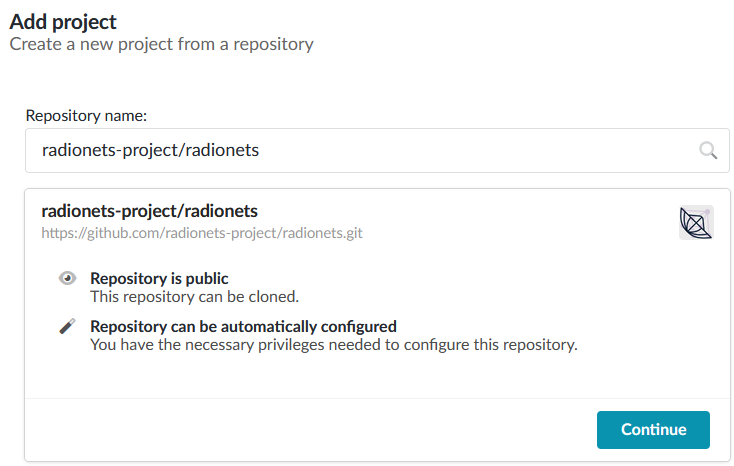
\includegraphics[width=\textwidth]{graphics/rtd2.png}
      }
      \only<4>{
        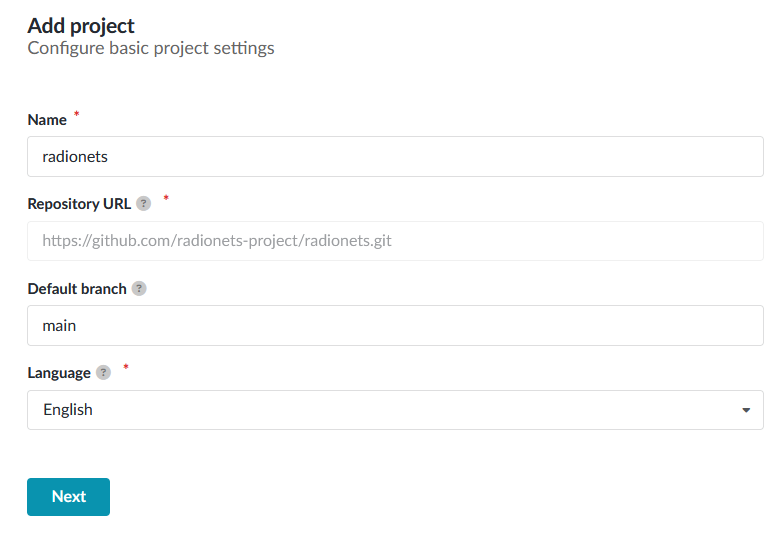
\includegraphics[width=\textwidth]{graphics/rtd3.png}
      }
      \only<5>{
        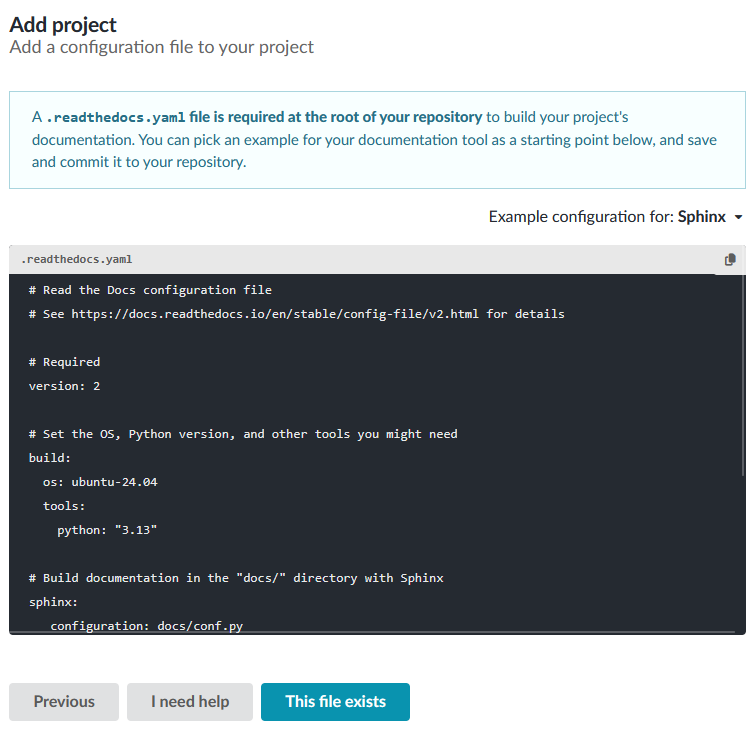
\includegraphics[width=\textwidth]{graphics/rtd4.png}
      }
      \only<6>{
        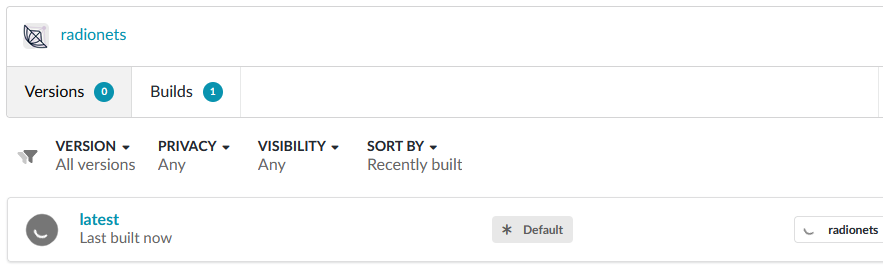
\includegraphics[width=\textwidth]{graphics/rtd5.png}
      }
    \end{column}
  \end{columns}
\end{frame}
